% Options for packages loaded elsewhere
\PassOptionsToPackage{unicode}{hyperref}
\PassOptionsToPackage{hyphens}{url}
\PassOptionsToPackage{dvipsnames,svgnames,x11names}{xcolor}
%
\documentclass[
  letterpaper,
  DIV=11,
  numbers=noendperiod]{scrartcl}

\usepackage{amsmath,amssymb}
\usepackage{iftex}
\ifPDFTeX
  \usepackage[T1]{fontenc}
  \usepackage[utf8]{inputenc}
  \usepackage{textcomp} % provide euro and other symbols
\else % if luatex or xetex
  \usepackage{unicode-math}
  \defaultfontfeatures{Scale=MatchLowercase}
  \defaultfontfeatures[\rmfamily]{Ligatures=TeX,Scale=1}
\fi
\usepackage{lmodern}
\ifPDFTeX\else  
    % xetex/luatex font selection
\fi
% Use upquote if available, for straight quotes in verbatim environments
\IfFileExists{upquote.sty}{\usepackage{upquote}}{}
\IfFileExists{microtype.sty}{% use microtype if available
  \usepackage[]{microtype}
  \UseMicrotypeSet[protrusion]{basicmath} % disable protrusion for tt fonts
}{}
\makeatletter
\@ifundefined{KOMAClassName}{% if non-KOMA class
  \IfFileExists{parskip.sty}{%
    \usepackage{parskip}
  }{% else
    \setlength{\parindent}{0pt}
    \setlength{\parskip}{6pt plus 2pt minus 1pt}}
}{% if KOMA class
  \KOMAoptions{parskip=half}}
\makeatother
\usepackage{xcolor}
\setlength{\emergencystretch}{3em} % prevent overfull lines
\setcounter{secnumdepth}{-\maxdimen} % remove section numbering
% Make \paragraph and \subparagraph free-standing
\ifx\paragraph\undefined\else
  \let\oldparagraph\paragraph
  \renewcommand{\paragraph}[1]{\oldparagraph{#1}\mbox{}}
\fi
\ifx\subparagraph\undefined\else
  \let\oldsubparagraph\subparagraph
  \renewcommand{\subparagraph}[1]{\oldsubparagraph{#1}\mbox{}}
\fi


\providecommand{\tightlist}{%
  \setlength{\itemsep}{0pt}\setlength{\parskip}{0pt}}\usepackage{longtable,booktabs,array}
\usepackage{calc} % for calculating minipage widths
% Correct order of tables after \paragraph or \subparagraph
\usepackage{etoolbox}
\makeatletter
\patchcmd\longtable{\par}{\if@noskipsec\mbox{}\fi\par}{}{}
\makeatother
% Allow footnotes in longtable head/foot
\IfFileExists{footnotehyper.sty}{\usepackage{footnotehyper}}{\usepackage{footnote}}
\makesavenoteenv{longtable}
\usepackage{graphicx}
\makeatletter
\def\maxwidth{\ifdim\Gin@nat@width>\linewidth\linewidth\else\Gin@nat@width\fi}
\def\maxheight{\ifdim\Gin@nat@height>\textheight\textheight\else\Gin@nat@height\fi}
\makeatother
% Scale images if necessary, so that they will not overflow the page
% margins by default, and it is still possible to overwrite the defaults
% using explicit options in \includegraphics[width, height, ...]{}
\setkeys{Gin}{width=\maxwidth,height=\maxheight,keepaspectratio}
% Set default figure placement to htbp
\makeatletter
\def\fps@figure{htbp}
\makeatother

\KOMAoption{captions}{tableheading}
\makeatletter
\@ifpackageloaded{tcolorbox}{}{\usepackage[skins,breakable]{tcolorbox}}
\@ifpackageloaded{fontawesome5}{}{\usepackage{fontawesome5}}
\definecolor{quarto-callout-color}{HTML}{909090}
\definecolor{quarto-callout-note-color}{HTML}{0758E5}
\definecolor{quarto-callout-important-color}{HTML}{CC1914}
\definecolor{quarto-callout-warning-color}{HTML}{EB9113}
\definecolor{quarto-callout-tip-color}{HTML}{00A047}
\definecolor{quarto-callout-caution-color}{HTML}{FC5300}
\definecolor{quarto-callout-color-frame}{HTML}{acacac}
\definecolor{quarto-callout-note-color-frame}{HTML}{4582ec}
\definecolor{quarto-callout-important-color-frame}{HTML}{d9534f}
\definecolor{quarto-callout-warning-color-frame}{HTML}{f0ad4e}
\definecolor{quarto-callout-tip-color-frame}{HTML}{02b875}
\definecolor{quarto-callout-caution-color-frame}{HTML}{fd7e14}
\makeatother
\makeatletter
\@ifpackageloaded{caption}{}{\usepackage{caption}}
\AtBeginDocument{%
\ifdefined\contentsname
  \renewcommand*\contentsname{Table of contents}
\else
  \newcommand\contentsname{Table of contents}
\fi
\ifdefined\listfigurename
  \renewcommand*\listfigurename{List of Figures}
\else
  \newcommand\listfigurename{List of Figures}
\fi
\ifdefined\listtablename
  \renewcommand*\listtablename{List of Tables}
\else
  \newcommand\listtablename{List of Tables}
\fi
\ifdefined\figurename
  \renewcommand*\figurename{Figure}
\else
  \newcommand\figurename{Figure}
\fi
\ifdefined\tablename
  \renewcommand*\tablename{Table}
\else
  \newcommand\tablename{Table}
\fi
}
\@ifpackageloaded{float}{}{\usepackage{float}}
\floatstyle{ruled}
\@ifundefined{c@chapter}{\newfloat{codelisting}{h}{lop}}{\newfloat{codelisting}{h}{lop}[chapter]}
\floatname{codelisting}{Listing}
\newcommand*\listoflistings{\listof{codelisting}{List of Listings}}
\makeatother
\makeatletter
\makeatother
\makeatletter
\@ifpackageloaded{caption}{}{\usepackage{caption}}
\@ifpackageloaded{subcaption}{}{\usepackage{subcaption}}
\makeatother
\ifLuaTeX
  \usepackage{selnolig}  % disable illegal ligatures
\fi
\usepackage[]{natbib}
\bibliographystyle{plainnat}
\IfFileExists{bookmark.sty}{\usepackage{bookmark}}{\usepackage{hyperref}}
\IfFileExists{xurl.sty}{\usepackage{xurl}}{} % add URL line breaks if available
\urlstyle{same} % disable monospaced font for URLs
\hypersetup{
  pdftitle={Solar wind discontinuities},
  colorlinks=true,
  linkcolor={blue},
  filecolor={Maroon},
  citecolor={Blue},
  urlcolor={Blue},
  pdfcreator={LaTeX via pandoc}}

\title{Solar wind discontinuities}
\usepackage{etoolbox}
\makeatletter
\providecommand{\subtitle}[1]{% add subtitle to \maketitle
  \apptocmd{\@title}{\par {\large #1 \par}}{}{}
}
\makeatother
\subtitle{FINESST23 Proposal}
\author{Zijin Zhang \and Anton V. Artemyev \and Vassilis
Angelopoulos \and Xiaofei Shi \and Ivan Vasko}
\date{2024-01-22}

\begin{document}
\maketitle

\section{Scientific/Technical/Management}\label{scientifictechnicalmanagement}

\subsection{Summary}\label{summary}

Rapid variations in interplanetary magnetic fields, commonly recognized
as solar wind magnetic discontinuities, embody important localized
transient rotations or jumps of the magnetic field. Considered
responsible for effective plasma heating, they carry the most intense
currents found in the solar wind. Theoretical models suggest that the
formation and destruction of discontinuities are closely related to the
nonlinear dynamics of Alfvén waves. These nonlinear processes can create
significant isolated disturbances to the otherwise adiabatic evolution
of the solar wind flow with a frozen interplanetary magnetic field. As
such, a comprehensive study of these discontinuities will considerably
enhance our understanding of the solar wind heating phenomenon.

Research into discontinuities in the solar wind begin with the onset of
the spacecraft era in the 1960s. This field of study has recently seen a
significant intensification, thanks to the launch of the Parker Solar
Probe (PSP), which enables magnetic field measurements at closer radial
distances to the Sun. Though discontinuities are found nearly everywhere
in the heliosphere (as shown by Voyager and Ulysses observations), the
most in-depth investigations have focused on the inner heliosphere,
around \(1\) astronomical unit (AU). \textbf{The primary aim of this
project is to utilize two novel datasets procured from PSP and Juno
magnetic field measurements, examining the evolution of discontinuity
properties within and far beyond 1 AU, up to Jupiter's orbit}. In
particular, we will generate and scrutinize two significant datasets:
\textbf{the first dataset} will collate \(1\) AU measurements from
STEREO, near-Earth WIND, and ARTEMIS missions with measurements beyond
\(1\) AU by Juno; \textbf{the second dataset} will amalgamate \(1\) AU
measurements with those made by PSP within \(1\) AU. The scientific
objective of this project is to answer the following three queries:

\begin{enumerate}
\def\labelenumi{\arabic{enumi}.}
\item
  How does the occurrence rate of discontinuity evolve with the radial
  distance \emph{beyond} \(1\) AU?
\item
  How does the occurrence rate of discontinuity evolve with the radial
  distance \emph{within} \(1\) AU?
\item
  How do various discontinuity characteristics, such as the magnetic
  field magnitude, current density, spatial scale, etc., evolve through
  the solar wind propagation from the near-Sun regions to 1AU, and
  subsequently to 5AU?
\end{enumerate}

To address the first question, we will integrate Juno measurements
between \(1\) and \(5\) AU with those at \(1\) AU, thereby
distinguishing temporal (correlated with solar activity) and spatial
(correlated with radial distance) variations in occurrence rates. The
same procedure will be utilized for PSP and \(1\) AU measurements to
address the second question. To respond to the third question,
information of solar wind velocity is requisite - these measurements are
available for all missions, except Juno, which does not activate plasma
instruments during the cruise to Jupiter. On a global scale, however,
the radial plasma speed of the expanding solar wind remains conserved,
hence we will use near-Earth solar wind measurements and a
Two-Dimensional Outer Heliosphere Solar Wind Modeling (MSWIM2D) of solar
wind propagation to reconstruct the solar wind velocity adjacent to
Juno's location.

\subsection{Significance of Investigation and Expected
Impact}\label{significance-of-investigation-and-expected-impact}

Spacecraft investigations of the space plasma environment has revealed
that the solar wind magnetic field only on average follows the Parker
model of the heliospheric current sheet. Localized transient currents,
that can be significantly more intense than the model currents, are
carried by various discontinuities observed as strong variations in
magnetic field components
\citep{colburn1966, burlagaMicroScaleStructuresInterplanetary1968, turnerOrientationsRotationalTangential1971}.
Most often such variations present as magnetic field rotation within the
plane of two most fluctuating components. As illustrated in
Figure~\ref{fig-1}, these rotations are observed at a multitude of
radial distances from the Sun. These discontinuities play an important
role in energy dissipation \citep[particle acceleration in the solar
wind,
see][]{dmitrukTestParticleEnergization2004, macbrideTurbulentCascadeAU2008, osmanIntermittencyLocalHeating2012, tesseinAssociationSuprathermalParticles2013}.
Moreover, they contribute significantly to magnetic fluctuation spectra
\citep{borovskyContributionStrongDiscontinuities2010, zhdankinMagneticDiscontinuitiesMagnetohydrodynamic2012, lionCoherentEventsSpectral2016}
and can affect space weather
\citep{tsurutaniReviewInterplanetaryDiscontinuities2011}. However,
previous observations of solar wind discontinuities in the deep space
rarely were conjugated with solar wind measurements closer to the Sun,
and thus did not provide a full picture of the structure and dynamics of
discontinuities. Juno magnetic field measurements over six years
(2011-2016) and PSP magnetic field and plasma measurements over four
years (2019-2023), in combination of STEREO, WIND, and ARTEMIS magnetic
field and plasma monitor at \(1\) AU during the operation of Juno and
PSP, provide a unique breakthrough datasets for the investigation of
discontinuities characteristics in both the inner and outer heliosphere.

\begin{wrapfigure}{r}{0.55\textwidth}

\centering{

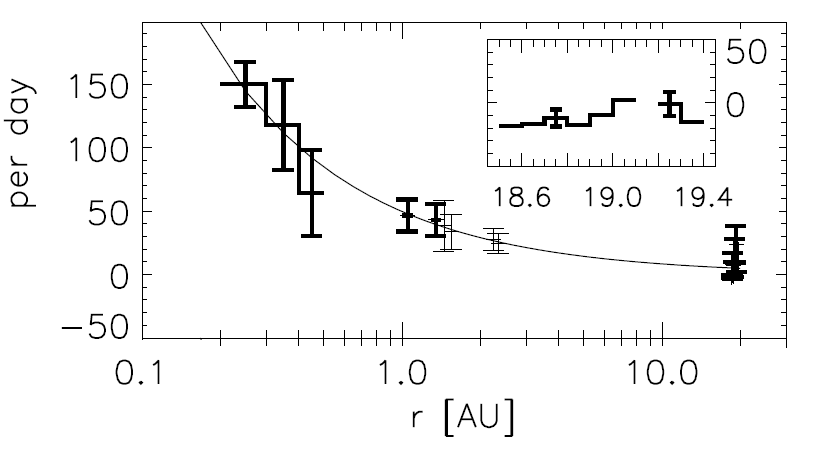
\includegraphics{figures/schematic.png}

}

\caption{\label{fig-1}Distribution of occurrence rate of solar wind
discontinuities \citep{sodingRadialLatitudinalDependencies2001}.}

\end{wrapfigure}%

Several heliospheric spacecraft missions have yielded statistical
information about the properties and potential origins of solar wind
discontinuities. For instance, Helios-1 and -2 observations showed an
abundance of discontinuities within the Earth's orbit (\(<1\) AU from
the Sun) \citep{Mariani83}. Similarly, Ulysses detected discontinuities
between 1 and 5 AU \citep{tsurutaniNonlinearElectromagneticWaves1997},
while Voyager 1's findings at \(39-43\) AU \citep{Burlaga96,Burlaga11}
suggested that these discontinuities pervade the entire heliosphere.
Combination of Voyager, Ulysses, WIND, and Helios-2 measurements of
discontinuities allows to reconstruct the radial variation of their
occurrence rate {[}see Figure~\ref{fig-1} and
\citep{sodingRadialLatitudinalDependencies2001}{]}, although
measurements at different radial distances were significantly separate
in time. Using simultaneous Juno, STEREO, WIND, and ARTEMIS or PSP,
STEREO, WIND, and ARTEMIS measurements, we will be able to investigate
and quantify the properties of \textbf{solar wind discontinuities at
different distances from the Sun, both within \(1\) AU and up to \(5\)
AU}.

Ulysses measurements of the high-latitude solar wind at \(1-5\) AU
showed that the majority of discontinuities resided within the
stream-stream interaction regions and/or within Alfvén wave trains
\citep{Tsurutani95, Tsurutani&Ho99}. The nonlinear evolution of Alfvén
waves (wave steepening) can be the main cause of such discontinuities.
The background plasma/magnetic field inhomogeneities and various
dissipative processes are key to Alfvén wave nonlinear evolution
\citep{Lerche75, Prakash&Diamond99, Medvedev97:prl, Nariyuki14, Yang15}.
In hybrid simulations
\citep[see][]{Vasquez&Hollweg98, Vasquez&Hollweg01, TenBarge&Howes13}
and analytical models
\citep[e.g.,][]{Kennel88:jetp, Hada89, Malkov91, Wu&Kennel92, Medvedev97:pop},
this steepening was shown to cause formation of discontinuities in
configurations resembling the near-Earth observations. There are models
predicting discontinuity formation
\citep{Servidio15, Podesta&Roytershteyn17} and destruction
\citep{Servidio11,Matthaeus15} due to dissipative processes (e.g.,
Alfvén wave steepening, magnetic reconnection) in the solar wind.
However, efficiency of these processes in realistic expanding solar wind
was not yet tested against observations. Regular and long-lasting Juno
and PSP observations together with almost permanent near-Earth solar
wind monitoring provide a unique opportunity to estimate discontinuity
occurrence rates over an unprecedentedly large radial distance range
(\(\sim 0.1\) AU - \(\sim 45\) AU). We will determine the discontinuity
occurrence rates for various radial distances and compare this rate with
the prediction of the adiabatic expansion model, \textbf{to understand
if discontinuity formation or destruction dominate the statistics of
discontinuities far away from the solar wind acceleration region}.

\subsection{Science Objectives and
Methodology}\label{science-objectives-and-methodology}

The main objective of this research is the examination of how solar wind
discontinuities evolve with radial distance. The methodology involves
the collection and analysis of two datasets: one that combines \(1\) AU
solar wind measurements conducted by STEREO, ARTEMIS, and WIND,
alongside Juno spacecraft measurements during its voyage from \(1\) AU
to \(5\) AU. The second dataset merges data from the same missions at
\(1\) AU and includes information from the PSP within the inner
heliosphere. This methodology will enable us to explore the following
research objectives:

\begin{enumerate}
\def\labelenumi{\arabic{enumi}.}
\item
  How does the occurrence rate of discontinuity evolve with the radial
  distance \emph{within} \(1\) AU and \emph{beyond} \(1\) AU?
\item
  How do various discontinuity characteristics, such as the magnetic
  field magnitude, current density, spatial scale, etc., evolve through
  the solar wind propagation from the inner heliosphere to outer
  heliosphere?
\end{enumerate}

In the next sections we briefly demonstrate preliminary results of this
project and basic elements of the project methodology.

\subsection{Demonstration of Project
Approaches}\label{demonstration-of-project-approaches}

\subsubsection{Dataset, spacecraft instruments, and solar wind
model}\label{dataset-spacecraft-instruments-and-solar-wind-model}

In this project we will use datasets of five missions measuring solar
wind magnetic field and plasma. Synergistic observations of these
missions should advance our understanding of the solar wind
discontinuities, their radial distribution and evolution
\citep{velli2020}.

\begin{SCfigure}

\centering{

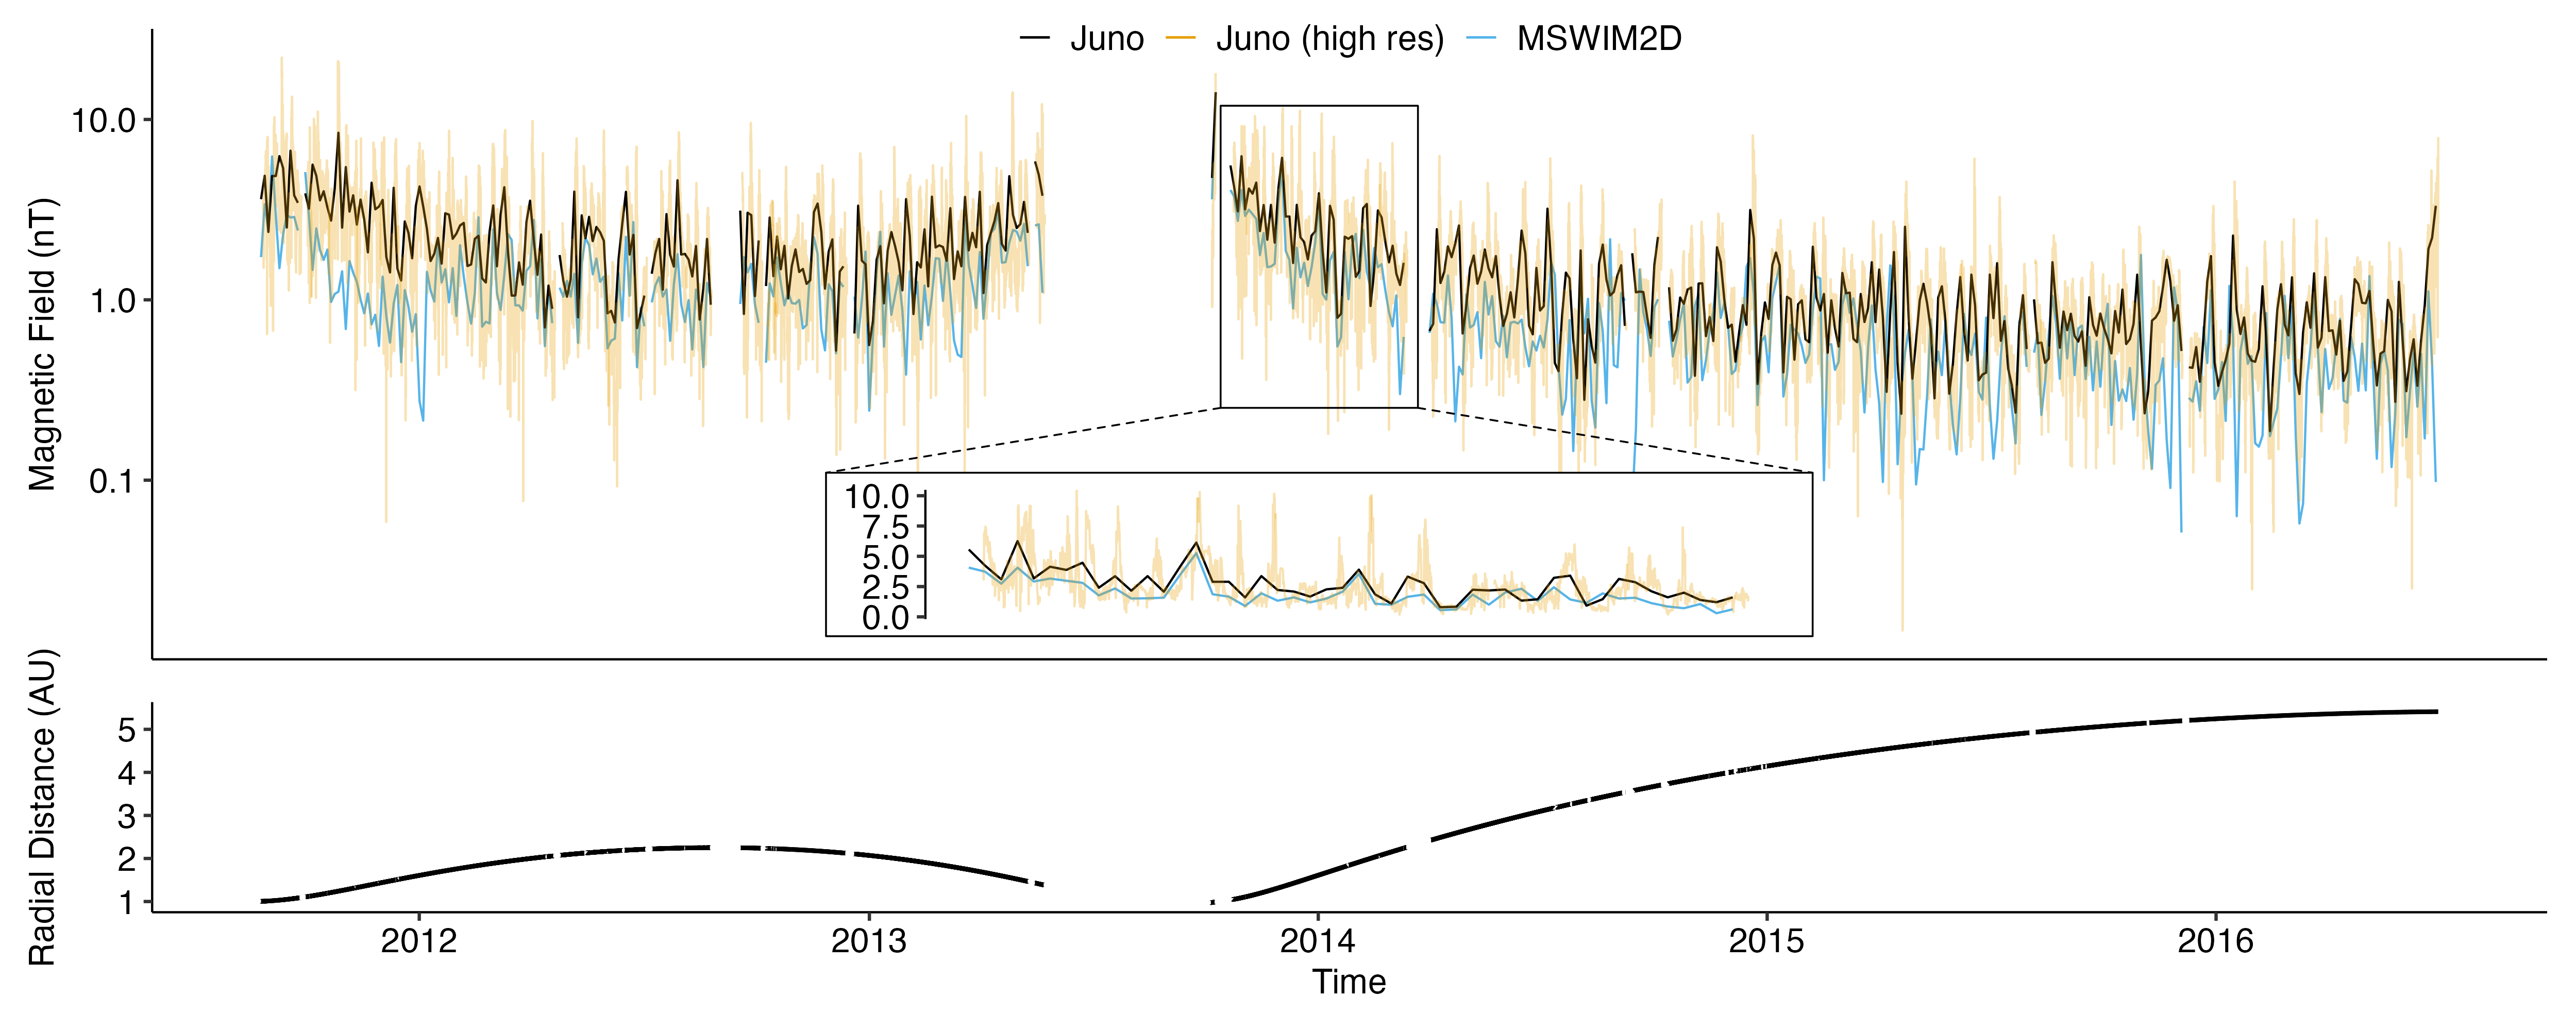
\includegraphics[width=0.75\textwidth,height=\textheight]{figures/juno_model_validation.png}

}

\caption{\label{fig-model}Time-series comparison of MSWIM2D (red) and
Juno-observed solar wind magnetic field magnitudes.}

\end{SCfigure}%

\paragraph{Juno}\label{juno}

We use the following data collected by Juno: magnetic fields with a
\(\sim1\) s resolution measured by the Juno Fluxgate Magnetometer (MAG)
\citep{connerney2017}, the ion bulk velocity \(v\), and the plasma
density \(n\) with a hourly resolution from solar wind model (see
below).

\paragraph{Parker Solar Probe (PSP)}\label{parker-solar-probe-psp}

We use the following data collected by PSP: magnetic fields measured by
the FIELDS experiment \citep{bale2016}, the ion bulk velocity \(v\), and
the plasma density \(n\) with a hourly resolution by the Solar Wind
Electrons Alphas and Protons (SWEAP) Investigation \citep{kasper2016}.

\paragraph{ARTEMIS}\label{artemis}

We use the following data collected by ARTEMIS: magnetic fields with a
\(\sim 1/5\) s resolution measured by the Fluxgate Magnetometer
\citep{auster2008}, the ion bulk velocity \(v\), and the plasma density
\(n\) calculated from velocity distribution by the Electrostatic
Analyzer with \(\sim 4\) s resolution \citep{mcfadden2009}.

\paragraph{STEREO}\label{stereo}

We use the following data collected by STEREO: magnetic fields with a
\(\sim1/8\) s resolution by the magnetic field experiment
\citep{acuña2008} on In-situ Measurements of Particles and CME
Transients (IMPACT) \citep{luhmann2008}, the ion bulk velocity \(v\),
and the plasma density \(n\) with a hourly resolution by the Plasma and
Suprathermal Ion Composition (PLASTIC) \citep{galvin2008}.

\paragraph{Wind}\label{wind}

We use the following data collected by Wind: magnetic fields with a
\(\sim 1/11\) s resolution measured by the Magnetic Field Investigation
(MFI) \citep{lepping1995}, the ion bulk velocity \(v\), and the plasma
density \(n\) with a hourly resolution by the Solar Wind Experiment
(SWE) \citep{ogilvie1995}.

\paragraph{Solar wind model}\label{solar-wind-model}

June measurements do not include plasma characteristics, and to estimate
discontinuity spatial scale (thicknesses) we will use solar wind speed
obtained from the model of solar wind propagation. The hourly solar wind
model data from the Two-Dimensional Outer Heliosphere Solar Wind
Modeling (MSWIM2D) \citep{keebler2022} will be employed to determine the
ion bulk velocity \(v\) and plasma density \(n\) at the location of the
Juno mission. Utilizing the BATSRUS MHD solver, this model is capable of
simulating the propagation of the solar wind from 1 to 75 astronomical
units (AU) in the ecliptic plane, effectively encompassing the region of
interest for our study. Figure \ref{fig-model} shows comparison of
magnetic field magnitudes obtained from MSWIM2D and measured by Juno.

\subsubsection{Determination of
discontinuities}\label{determination-of-discontinuities}

We will use \citet{liu2022a} method to identify discontinuities in the
solar wind. This method has better compatibility for the discontinuities
with minor field changes, and is more robust to the situation
encountered in the outer heliosphere. For each sampling instant \(t\),
we define three intervals: the pre-interval \([-1,-1/2]\cdot T+t\), the
middle interval \([-1/,1/2]\cdot T+t\), and the post-interval
\([1/2,1]\cdot T+t\), in which \(T\) are time lags. Let time series of
the magnetic field data in these three intervals are labeled
\({\bf B}_-\), \({\bf B}_0\), \({\bf B}_+\), respectively. Then for an
discontinuity, the following three conditions should be satisfied: (1)
\(\sigma({\bf B}_0)>2\max\left(\sigma({\bf B}_-, \sigma({\bf B}_+)\right)\),
(2)
\(\sigma\left({\bf B}_-+{\bf B}_+\right)>\sigma({\bf B}_-)+\sigma({\bf B}_+)\),
and (3) \(|\Delta {\bf B}|>|{\bf B}_{bf}|/10\), in which \(\sigma\) and
\({\bf B}_{bg}\) represent the standard deviation and the background
magnetic field magnitude, and
\(\Delta {\bf B}={\bf B}(t+T/2)-{\bf B}(t-T/2)\). The first two
conditions guarantee that the field changes of the discontinuity
identified are large enough to be distinguished from the stochastic
fluctuations on magnetic fields, while the third is a supplementary
condition to reduce the uncertainty of recognition. We also will use the
minimum or maximum variance analysis (MVA) analysis
\citep{sonnerupMinimumMaximumVariance1998, sonnerupMagnetopauseStructureAttitude1967}
to determine the main (most varying) magnetic field component, \(B_l\),
and medium variation component, \(B_m\). Figure~\ref{fig-examples} shows
several examples of solar wind discontinuities detected by different
spacecraft.

\begin{SCfigure}

\centering{

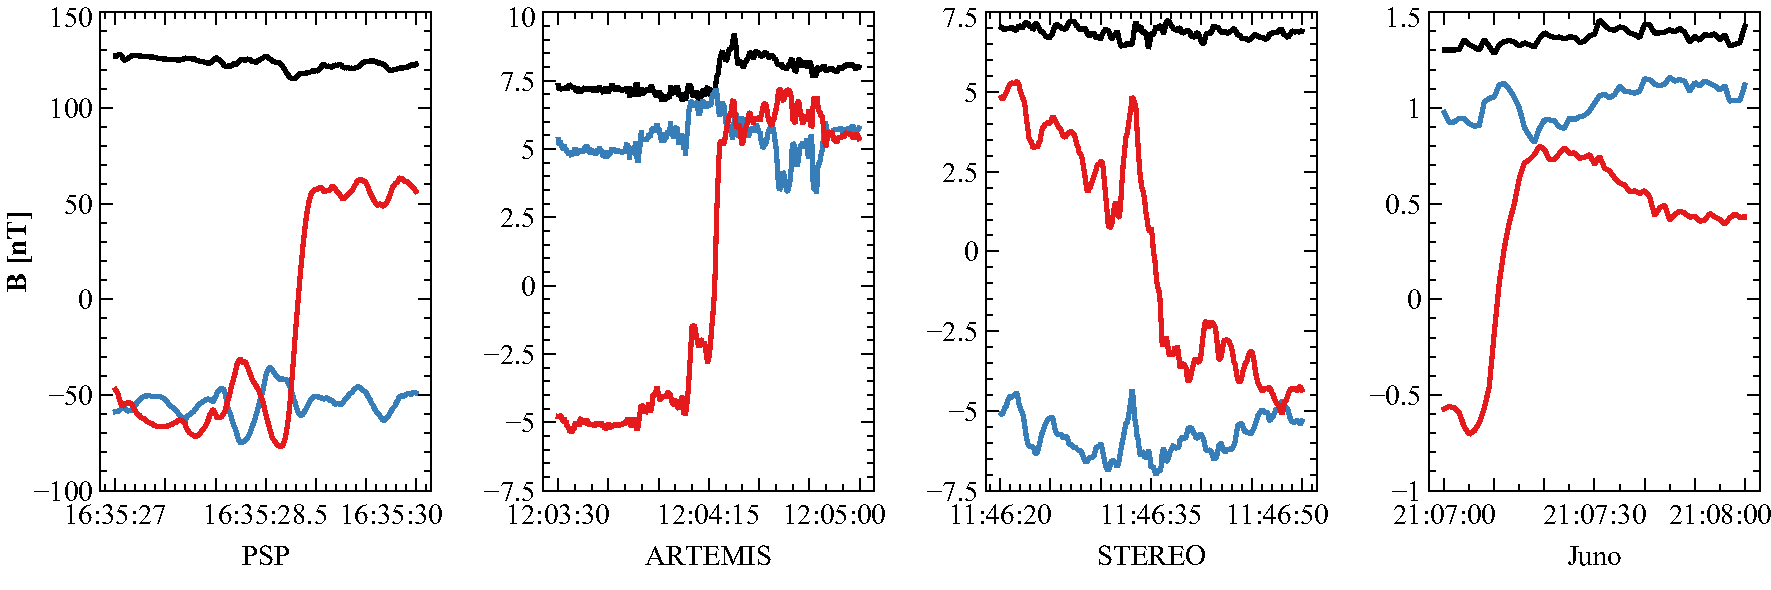
\includegraphics[width=0.75\textwidth,height=\textheight]{figures/fig-ids_examples.pdf}

}

\caption{\label{fig-examples}Discontinuities detected by PSP, Juno,
STEREO and near-Earth ARTEMIS satellite: red, blue, and black lines are
\(B_l\), \(B_m\), and \(|{\bf B}|\).}

\end{SCfigure}%

\subsubsection{Discontinuity occurrence
rate}\label{discontinuity-occurrence-rate}

The basic approach of this proposal is to use solar wind measurements at
1AU (STEREO, ARTEMIS, WIND) to compare with Juno and PSP measurements
and distinguish effects of solar wind temporal variations and effects of
spatial (with the radial distance from the Sun) variations of
discontinuity occurrence rate and characteristics. The example of such
comparison for the occurrence rate is shown in Fig. \ref{fig:rate},
where we plot number of discontinuities measured per day by different
spacecraft missions (for the same temporal resolution of magnetic field
data and the same criteria of discontinuity determination). The radial
distance of Juno for 2011-2015 is shown in Fig. \ref{fig-model}, and the
number of discontinuities measured by Juno per day coincides with the
discontinuity number measured by STEREO, WIND, and ARTEMIS, when Juno is
around \(1\) AU. This number (occurrence rate) decreases with distance
(with time after \(\sim 2013\)), as Juno moves from \(1\) AU to \(5\)
AU. We will use the similar comparison for discontinuity characteristics
and occurrence rate derived for PSP and Juno.

\begin{SCfigure}
{\centering 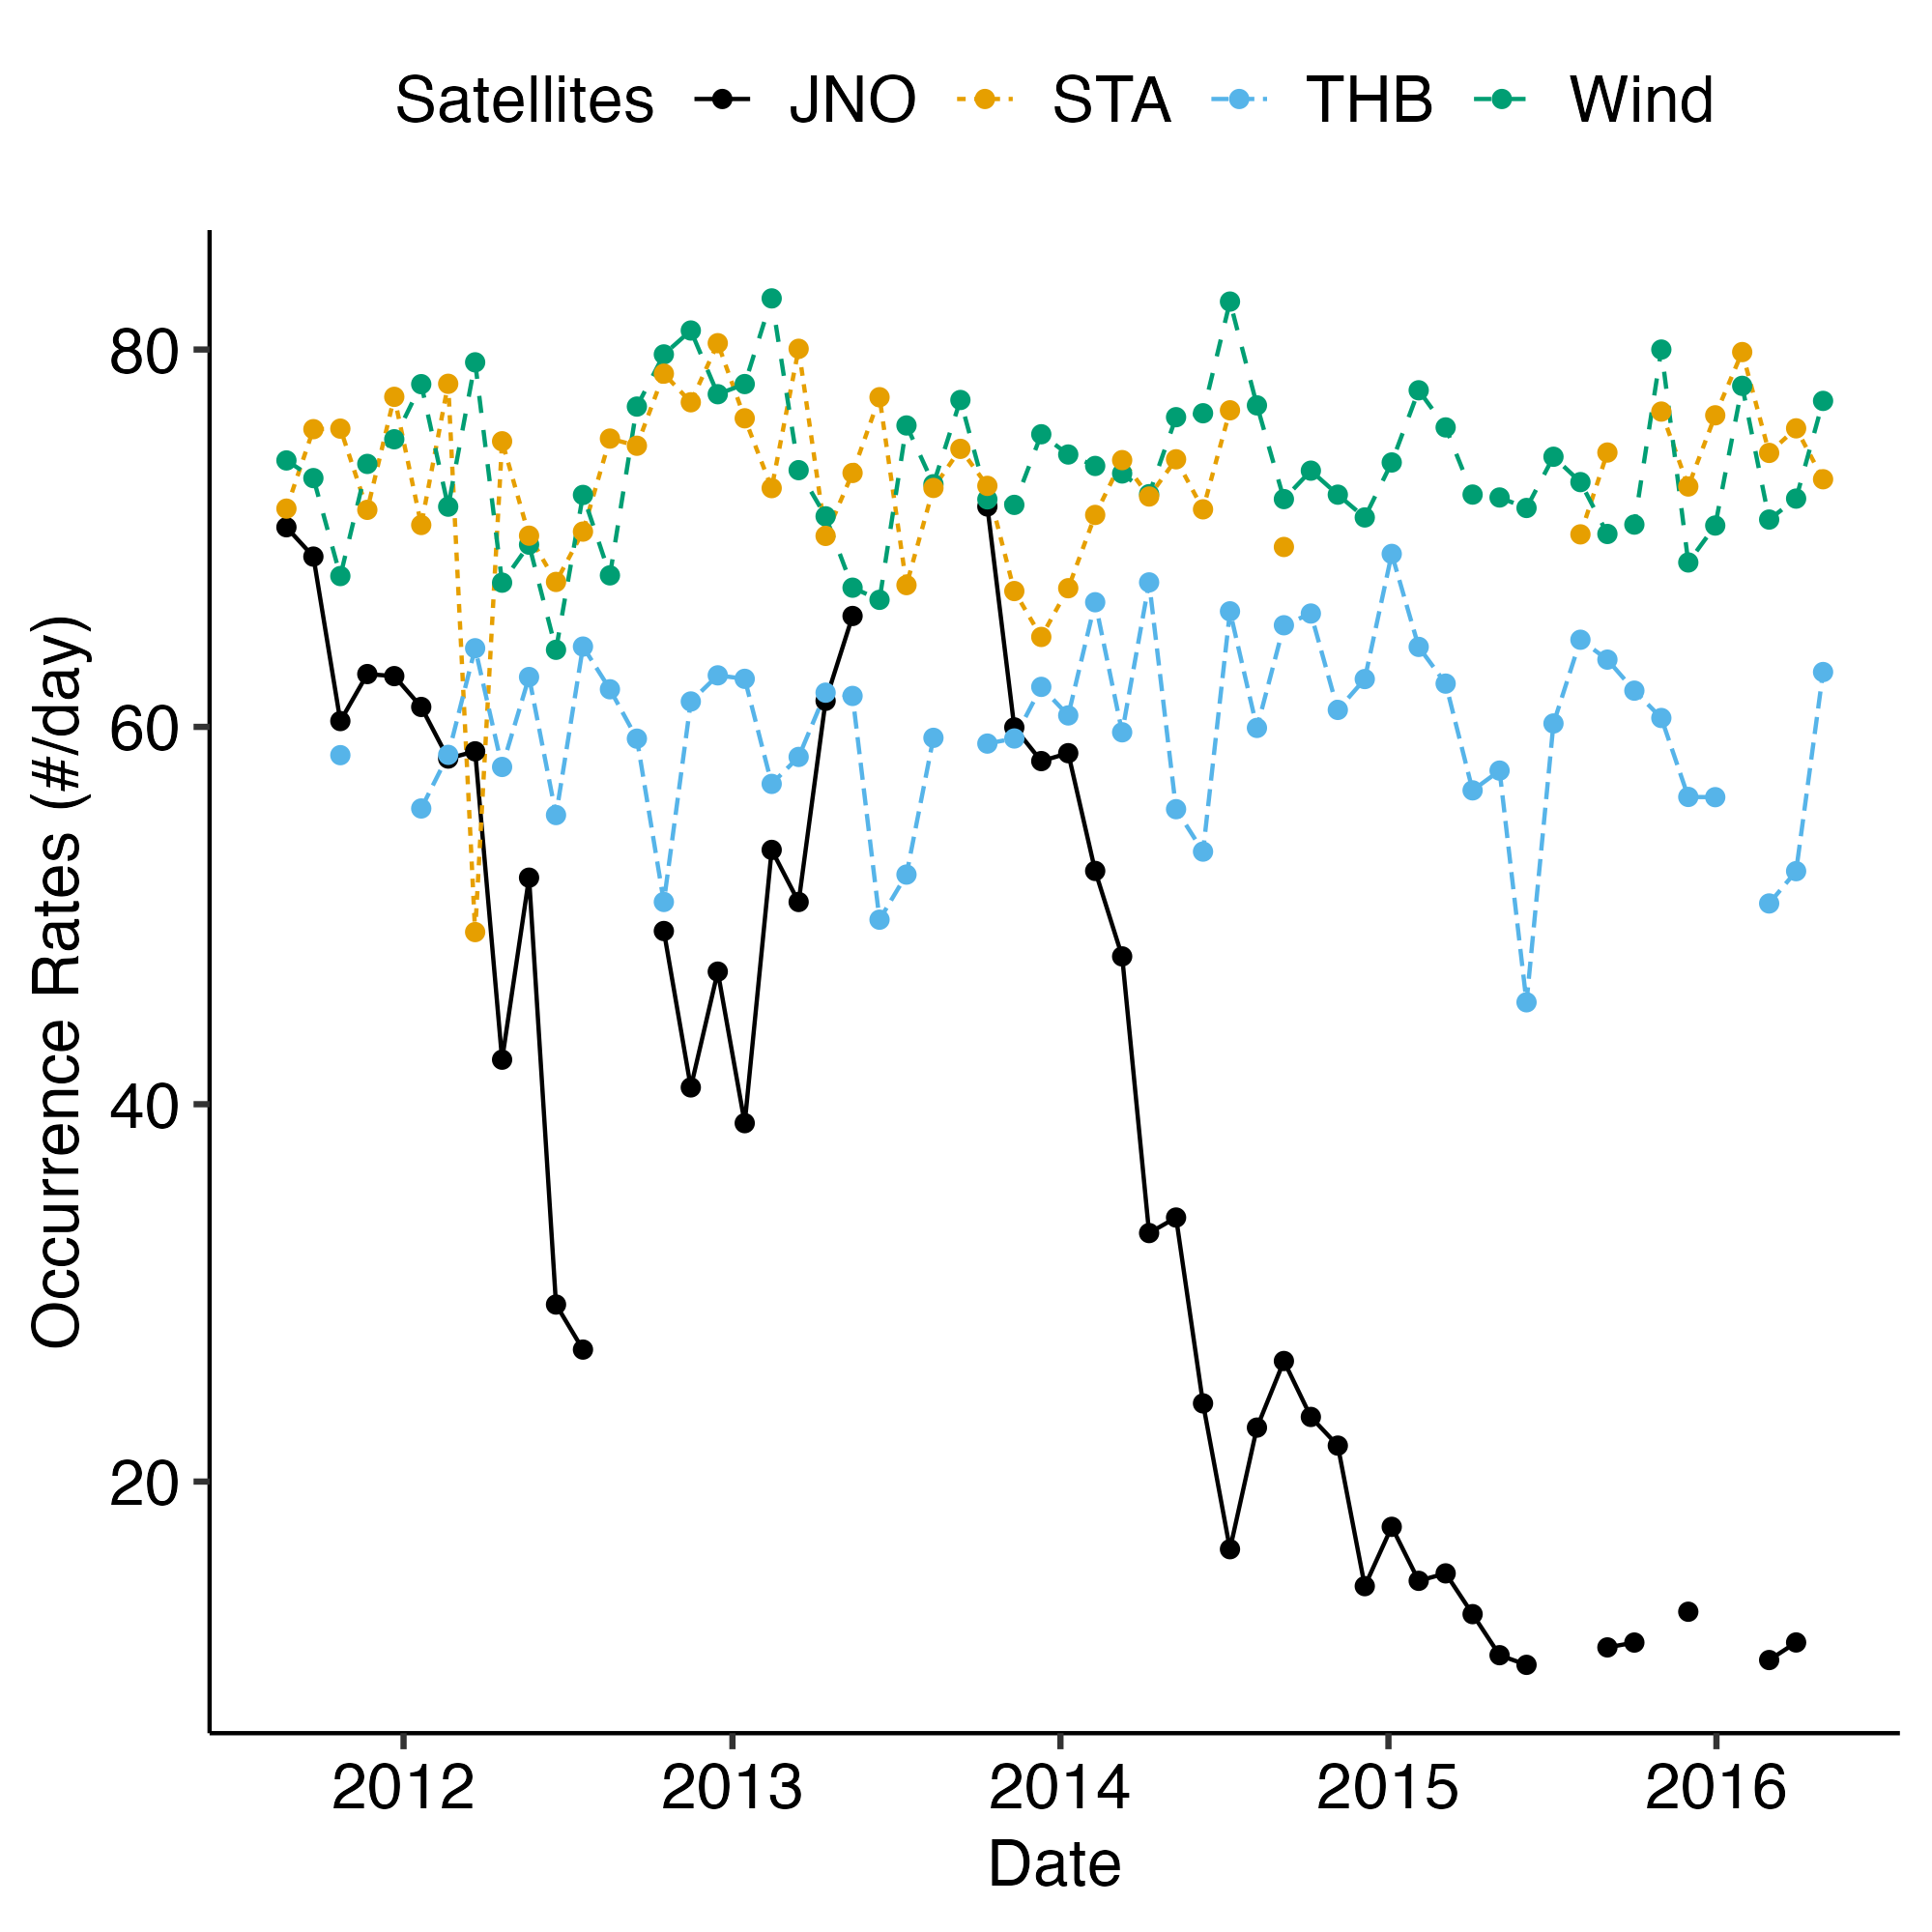
\includegraphics[width = 0.45\textwidth]{figures/ocr_time_cleaned.png}}
    \caption{The number of discontinuities measured by Juno per day coincides with the discontinuity number measured by STEREO, WIND, and ARTEMIS, when Juno is around $1$ AU. This number (occurrence rate) decreases with distance (with time after $\sim 2013$), as Juno moves from $1$ AU to $5$ AU. We will use the similar comparison for discontinuity characteristics and occurrence rate derived for PSP and Juno. The radial distance of Juno for 2011-2015 is shown in Fig. \ref{fig-model}.}
    \label{fig:rate}
\end{SCfigure}

\begin{SCfigure}

\centering{

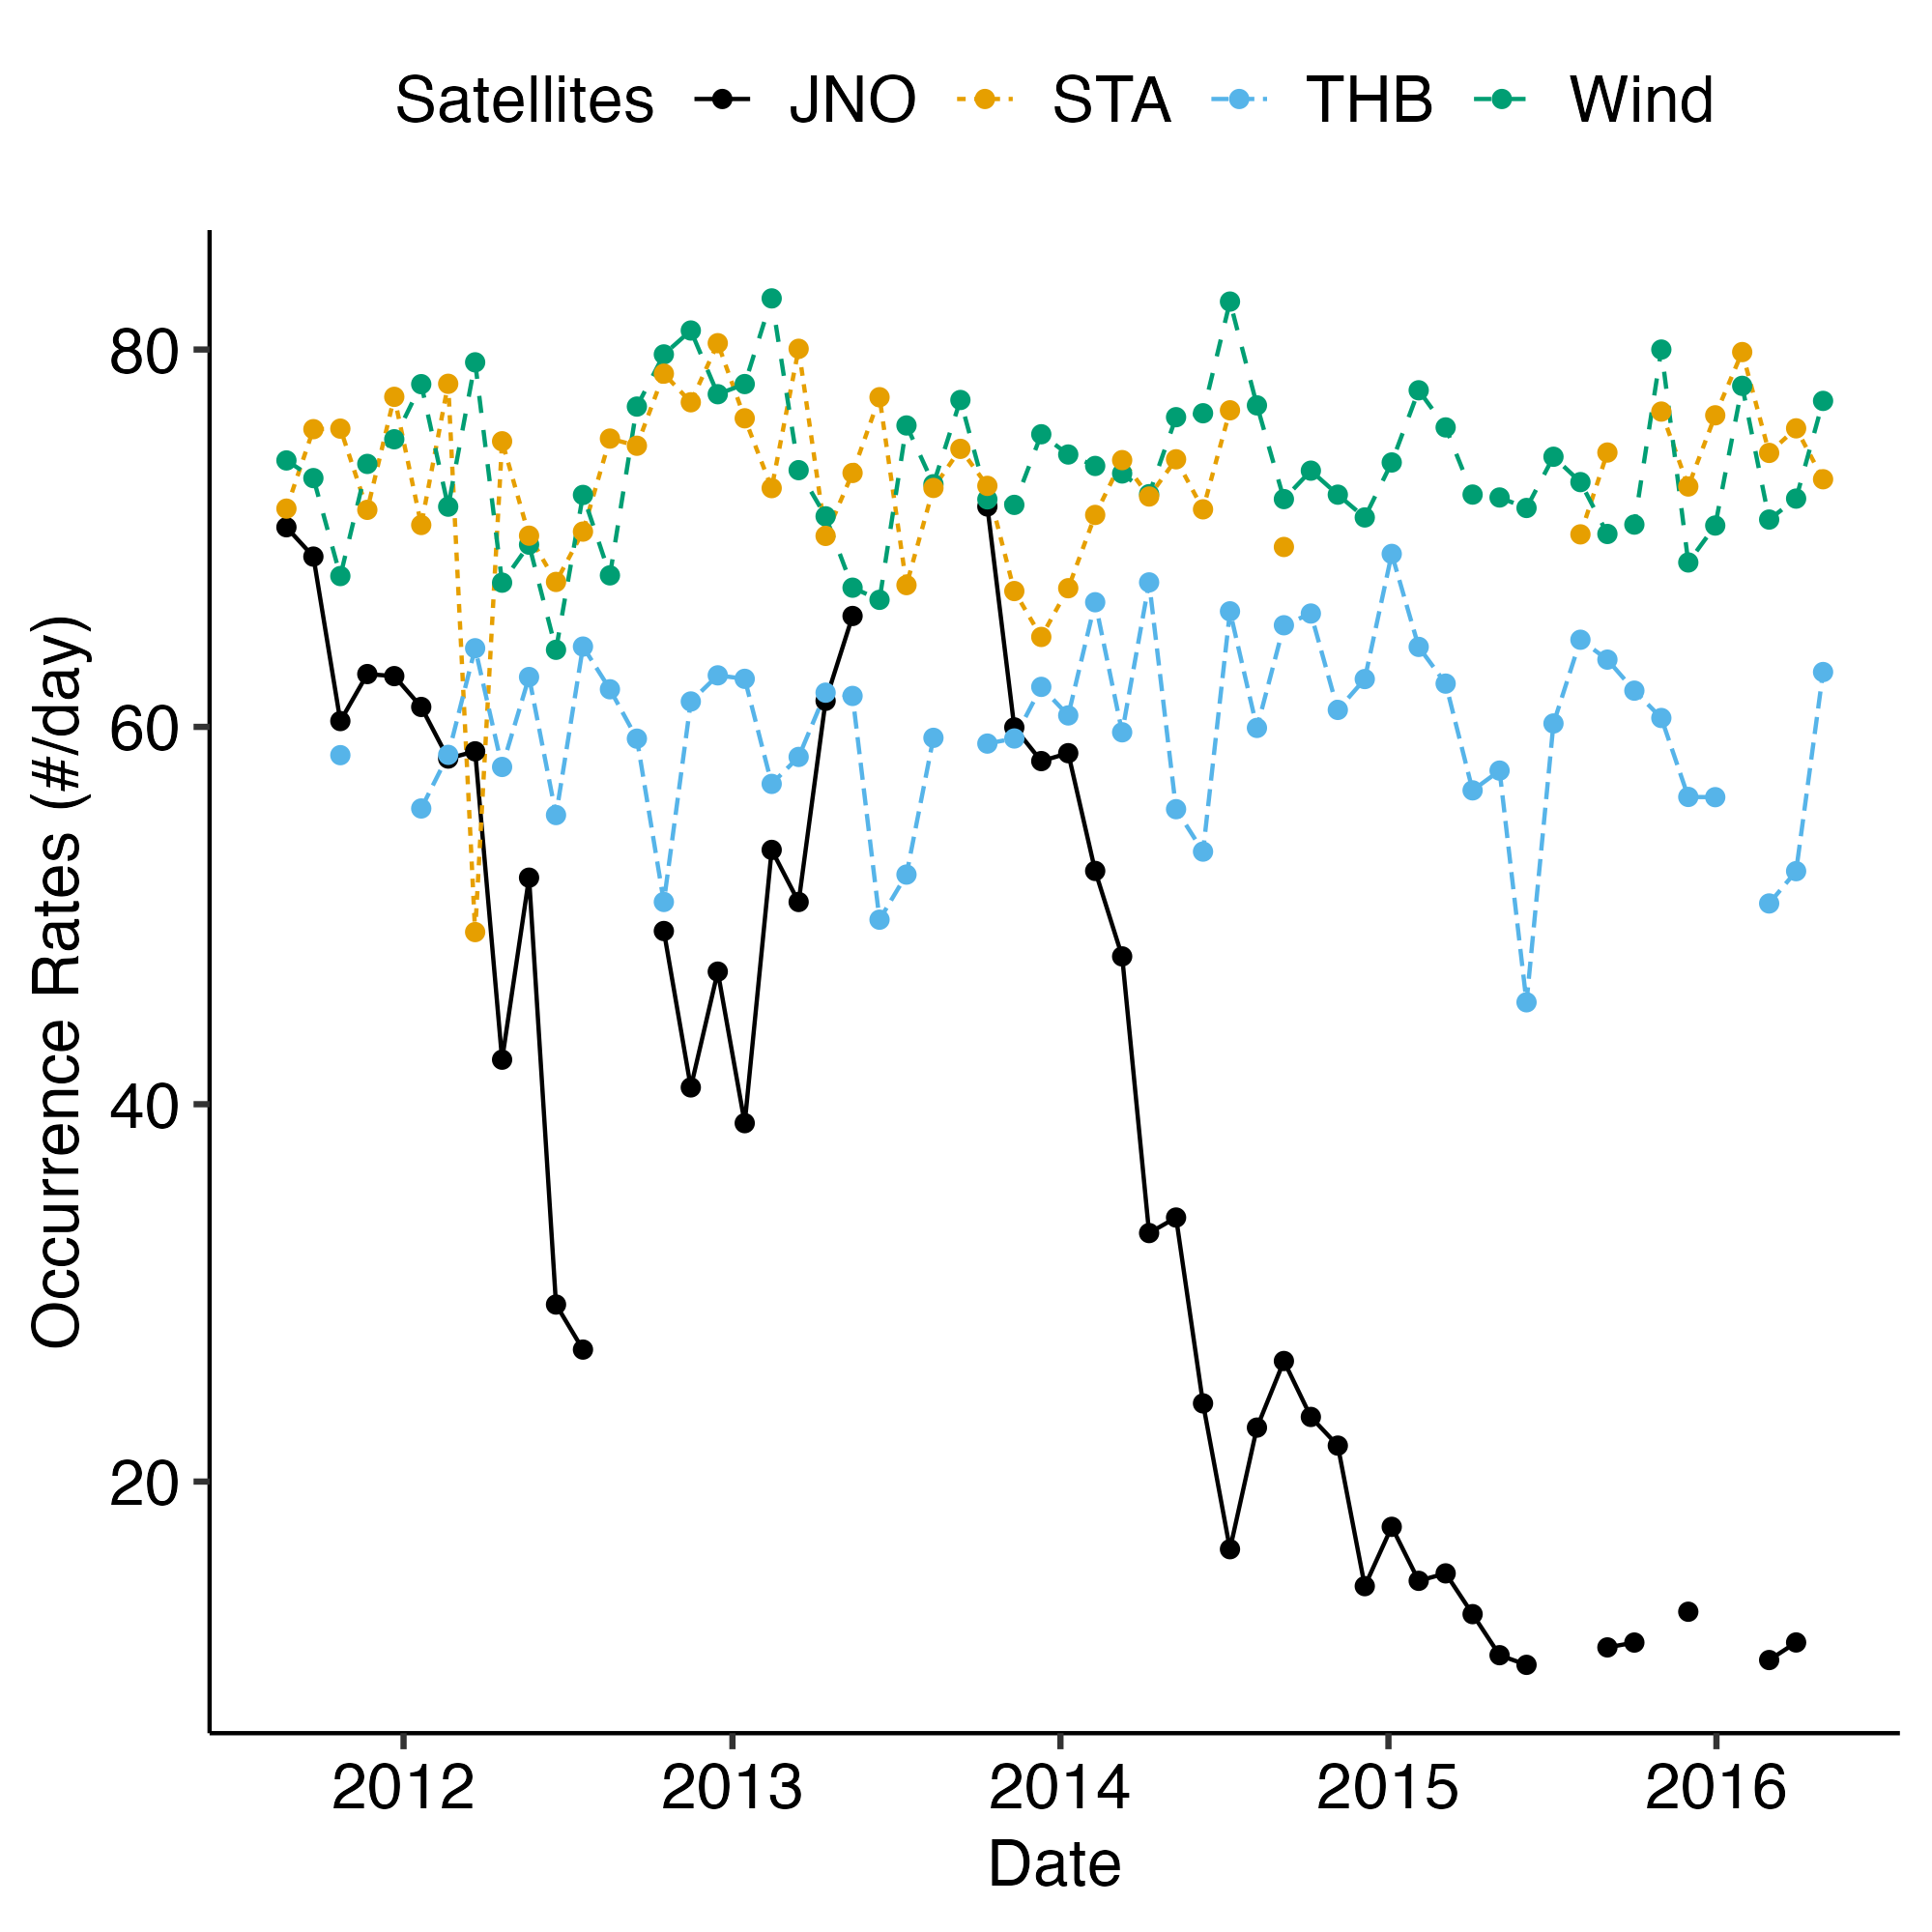
\includegraphics[width=0.45\textwidth,height=\textheight]{figures/ocr_time_cleaned.png}

}

\caption{\label{fig-rate}The number of discontinuities measured by Juno
per day coincides with the discontinuity number measured by STEREO,
WIND, and ARTEMIS, when Juno is around \(1\) AU. This number (occurrence
rate) decreases with distance (with time after \(\sim 2013\)), as Juno
moves from \(1\) AU to \(5\) AU. We will use the similar comparison for
discontinuity characteristics and occurrence rate derived for PSP and
Juno. The radial distance of Juno for 2011-2015 is shown in
Figure~\ref{fig-model}.}

\end{SCfigure}%

\subsection{Relevance to Heliophysics Overarching
Goal}\label{relevance-to-heliophysics-overarching-goal}

This project focuses on investigation of the solar wind discontinuities,
the key element of magnetic field turbulence and the primary interface
of charged particle acceleration. Thus, the project contributes to NASA
Heliophysics' overarching goal to: \emph{``Explore and characterize the
physical processes in the space environment from the Sun to the
heliopause and throughout the univers''} and its specific objectives to:
\emph{``Explore the physical processes at work in the space environment
from the Sun to Earth and throughout the solar system''}.

\subsection{Project Schedule}\label{project-schedule}

This project, spanning three years, assigns each year to a stated
objective: in the \textbf{first year}, the focus will be on compiling
and analyzing Juno's observations of solar wind discontinuities,
supported by a solar wind model and supplemental observations from \(1\)
AU missions (STEREO, ARTEMIS, WIND); in the \textbf{second year}, a
similar analysis of solar wind discontinuities will be conducted for
PSP, using additional data from the \(1\) AU missions. In the
\textbf{third year}, specific discontinuity characteristics, such as
spatial scales and current density, will be analyzed for both datasets.
The radial evolution of these features will be compared to the
expectations predicted from solar wind adiabatic expansion.

\paragraph{Management}\label{management}

of this project is fully performed by \textbf{FI}, Zijin Zhang, who will
also be responsible for the assembly and analysis of the observational
dataset, and generation of a combined Juno/solar wind model dataset.
Project \textbf{PI}, Prof.~Vassilis Angelopoulos, and group members
Dr.~Anton Artemyev and Dr.~Chen Shi, will contribute to discussions and
the education and training of Zijin Zhang. Expertise of Prof.~V.
Angelopoulos in spacecraft measurement techniques and data analysis
\cite{Angelopoulos19,Angelopoulos11:ARTEMIS}, Dr.~A. Artemyev in solar
wind discontinuity observation and modeling
\citep{Artemyev18:apj,Artemyev19:jgr:solarwind}, and Dr.~Chen Shi in
solar wind observations and simulations
\citep{ChenShi21:a&a,ChenShi22:apj,ChenShi23:apj} guarantees that Z.
Zhang will receive all necessary mentorship, advice and support, and
thus will successfully complete the thesis project.

\section{References and
Acknowledgements}\label{references-and-acknowledgements}

\renewcommand{\bibsection}{}
\bibliography{files/bibliography/addon_zijin.bib,files/references.bib,files/addon.bib}

\textbf{Acknowledgement}: This proposal is the work of the FI (Zijin
Zhang). PI (Vassilis Angelopoulos) and group members (Dr.~A. Artemyev,
Dr.~Chen Shi) provide editorial support (clarity and structure).

\section{Open Science and Data Management Plan
(OSDMP)}\label{open-science-and-data-management-plan-osdmp}

This project aims to develop two key outputs: a data product focusing on
the statistics of solar wind discontinuities and a suite of modeling
software for analyzing these phenomena.

\subsection{Data Products: Statistics of Solar Wind
Discontinuities}\label{data-products-statistics-of-solar-wind-discontinuities}

\paragraph{Product Description:}\label{product-description}

We will generate comprehensive statistics derived from in-situ satellite
measurements. This includes:

\begin{enumerate}
\def\labelenumi{\alph{enumi}.}
\tightlist
\item
  Event lists in ASCII format.
\item
  Parameters of solar wind discontinuities from two datasets: Juno
  observations (2011-2015) combined with \(1\)AU observations, and PSP
  observations combined with \(1\)AU observations.
\item
  Visual aids such as figures in PNG format and detailed tables in ASCII
  format, providing insights into solar wind velocity and density as
  reconstructed for the Juno location.
\end{enumerate}

\paragraph{Scientific Significance:}\label{scientific-significance}

This dataset will facilitate the first quantification of the evolution
of solar wind discontinuity with radial distance.

\paragraph{Data Types and Volume:}\label{data-types-and-volume}

The project will produce ASCII tables and figure files, estimated to be
less than 10 GB in total.

\paragraph{Documentation and
Delivery:}\label{documentation-and-delivery}

Comprehensive documentation, including selection criteria for solar wind
discontinuities and spacecraft measurement details, will be provided.
The expected delivery time is in the third year of the project.

\paragraph{Archiving Method:}\label{archiving-method}

The data products will be published as supporting information in
academic papers focused on solar wind discontinuity characteristics at
various radial distances. Additionally, the dataset will be uploaded to
the open archive \href{https://zenodo.org/}{Zenodo}.

\subsection{Software: Modular and Scalable Solutions for Solar Wind
Analysis}\label{software-modular-and-scalable-solutions-for-solar-wind-analysis}

\paragraph{Software Overview}\label{software-overview}

We are in the process of developing a set of routines that are both
modular and scalable, tailored specifically for in-depth solar wind
analysis and the identification of discontinuities. These routines,
accessible in Python and Interactive Data Language (IDL), are designed
with a focus on performance efficiency and adaptability, enabling the
analysis of data from diverse space missions. The initial Python library
is available at our \href{https://beforerr.github.io/ids_finder}{project
website}.

\paragraph{Scientific Significance:}\label{scientific-significance-1}

These advanced routines will not only facilitate detailed analysis of
solar wind discontinuities and their radial evolution but also provide a
comprehensive toolset for the broader scientific community to study
magnetic field data from various space missions.

\paragraph{Modular and Scalable
Design:}\label{modular-and-scalable-design}

The software's modular architecture allows for easy adaptation and
extension, making it suitable for analyzing data beyond the initial
scope of this project. Its scalable nature ensures efficient
performance, even when dealing with large datasets from different
missions.

\paragraph{Data Types and Volume:}\label{data-types-and-volume-1}

The software package will consist of IDL and Python files, collectively
amounting to less than 10 MB.

\paragraph{Documentation and Release:}\label{documentation-and-release}

We will provide comprehensive documentation, including detailed
descriptions of each module, usage guidelines, and examples. This
documentation will assist users in customizing the software for their
specific needs. The software is expected to be released in the first
year of the project.

\paragraph{Archiving Method:}\label{archiving-method-1}

Python function will be integrated into the open-source Python-based
Space Physics Environment Data Analysis System (PySPEDAS), while IDL
routines will be added to the SPEDAS framework \cite{Angelopoulos19}.
Both will be available under MIT license terms and also uploaded to
\href{https://zenodo.org/}{Zenodo}.

\subsection{Roles and responsibilities of team members for data
management}\label{roles-and-responsibilities-of-team-members-for-data-management}

The Project FI, with the guidance of the PI, will be responsible for
releasing and archiving all datasets produced within this project.

\subsection{Publication of results}\label{publication-of-results}

We anticipate producing 2-3 peer-reviewed manuscripts for journals such
as J. Geophys. Res. and Geophys. Res. Lett. Each manuscript will include
a supplementary dataset (as detailed in Section 1) to facilitate result
reproduction. Project funds will be utilized to ensure open access
publication of these papers.

\section{Research Readiness
Statement}\label{research-readiness-statement}

I believe I am well-prepared for the proposed research, drawing from
extensive academic and experiential learning in Space Science,
complemented by mentorship.

\subsection{Professional preparation}\label{professional-preparation}

My academic background includes core courses in physics and space
science at both undergraduate and graduate levels, such as
Electromagnetic Theory, Plasma Physics, and Solar System
Magnetohydrodynamics. This education forms a solid base for the proposed
study on solar wind discontinuities.

In addition to this, my mentors and I have developed a comprehensive
plan for my training and research. As part of this plan, I regularly set
aside time for self-study to delve deeper into the field and present
latest journal articles/review papers to stay updated on the latest
research. My mentors provides guidance, support, and resources to help
me enhance my research skills, carry out innovative investigations, and
present my findings effectively.

As for computer programming and data analysis tools, during my graduate
studies, I have become proficient in Python (PySPEDAS, PlanetaryPy,
Astropy, Plasmapy), IDL (SPEDAS, CDAS), Julia, and Mathematica. I have
used these tools in analyzing mission data from different projects,
including Juno, PSP, and THEMIS. I am confident in my ability to utilize
these tools effectively for the proposed study---particularly for
analyzing discontinuities in the solar wind and sorting through large
datasets from several missions.

\subsection{Graduate study timeline}\label{graduate-study-timeline}

I'm enrolled in a combined Master's and Ph.D.~program in Space Science
at UCLA since September 2022, with an anticipated graduation in August
2026. This timeline aligns well with the duration required for the
proposed research.

\subsection{Research experiences}\label{research-experiences}

My practical research skills stem from undergraduate work in the
Wave-particle Interactions Group and an internship at the National Space
Science Center. These experiences, including simulating solar wind
interactions and processing GNSS data, have sharpened my data analysis
and numerical modeling capabilities.

Further, I've engaged in self-directed learning through workshops,
conference student days and short summer courses, enhancing my
understanding of space weather and plasma dynamics. My roles as a
Teaching Assistant and president of the student scientific expedition
association have developed my communication, mentoring, and project
management skills, essential for collaborative research and
dissemination.

Overall, my diverse experiences and proactive learning initiatives
provide a strong foundation for conducting advanced analysis and
interpretation in space physics.

\section{Biographical Sketches/Curriculum Vitae
(CVs)}\label{biographical-sketchescurriculum-vitae-cvs}

\section{Current and Pending Support}\label{current-and-pending-support}

\begin{tcolorbox}[enhanced jigsaw, colback=white, opacityback=0, titlerule=0mm, opacitybacktitle=0.6, arc=.35mm, breakable, toprule=.15mm, colbacktitle=quarto-callout-note-color!10!white, bottomtitle=1mm, toptitle=1mm, leftrule=.75mm, coltitle=black, rightrule=.15mm, colframe=quarto-callout-note-color-frame, bottomrule=.15mm, left=2mm, title=\textcolor{quarto-callout-note-color}{\faInfo}\hspace{0.5em}{Note}]

Current and Pending (C\&P) Support has no page limits. FIs must
identify, when applicable, any external-to-the-proposing organization
funding, e.g., from U.S. federal, U.S. non-federal, and non-U.S. sources
or active applications for grants, fellowships etc., particularly those
that have overlap with the proposed work. All PIs, regardless of F.5-14
the time devoted to FINESST, likewise must report C\&P. There is no
template established for reporting this information and if the reviewing
Division has a template posted, such templates may be used, but are not
required. C\&P templates or forms in use by the proposing institution
are welcome. To make it clear to NASA when the FI and/or PI have no C\&P
to report, include a joint statement or separate statements, if
applicable, that there is ``No C\&P funding to report''.

\end{tcolorbox}

\section{Statements of Commitment and Letters of Resource
Support}\label{statements-of-commitment-and-letters-of-resource-support}

\begin{tcolorbox}[enhanced jigsaw, colback=white, opacityback=0, titlerule=0mm, opacitybacktitle=0.6, arc=.35mm, breakable, toprule=.15mm, colbacktitle=quarto-callout-note-color!10!white, bottomtitle=1mm, toptitle=1mm, leftrule=.75mm, coltitle=black, rightrule=.15mm, colframe=quarto-callout-note-color-frame, bottomrule=.15mm, left=2mm, title=\textcolor{quarto-callout-note-color}{\faInfo}\hspace{0.5em}{Note}]

Do not add Statements of Commitment from any team member listed under
Section VI of the NSPIRES cover page and who acknowledges commitment via
NSPIRES. For example, when a collaborator or Co-I directly confirms
their participation via NSPIRES, that is sufficient commitment. If the
proposing team has regular access to a facility or resource, then no
letter of Resource support is needed. See Section 2.17 in the 2023 NASA
Proposer's Guide for how to prepare ``Letters of Resource Support'\,' to
demonstrate that a facility or resource is available for the proposed
use. Statements of commitment are only required when commitment cannot
be made via NSPIRES, such as when a proposer is using Grants.gov.

\end{tcolorbox}

\section{Mentoring Plan or Agreement}\label{mentoring-plan-or-agreement}

Zijin Zhang is a 2nd year PhD student mentored by Prof.~Angelopoulos
(PI), and in the supportive and intellectually dynamic environment of
the Experimental Space Physics group that includes Dr.~Chen Shi and and
Dr.~Anton Artemyev. He is about to schedule his department oral exam,
defining his thesis topic on the subject proposal. He has demonstrated
independent research capabilities and creative work through the
presentations in several international science meetings. The Mentoring
Plan for Mr.~Zhang includes:

\begin{itemize}
\tightlist
\item
  Weekly individual (splinter) meetings with Prof.~Angelopoulos (PI),
  Dr.~Chen and Dr.~Artemyev. These are mostly to operationally resolve
  issues of the research plan realization and review the progress and
  work towards the stated goals.
\item
  Weekly updated in group meetings, that serve for quick opinion
  exchange with other team members (several experts on solar wind
  discontinuity) on hot-off-the-press results.
\item
  Splinter discussions with local experts on the observational and
  theoretical aspects of the project (Prof.~Velli: PSP dataset). These
  one-on-one meetings aim to provide additional training for Mr.~Zhang
  in data analysis techniques and theoretical approaches useful for
  project realization.
\end{itemize}

These research meetings plus presentations in joint inter-departmental
(encompassing AOS, P\&A and EPSS department members) space physics
student presentations, Journal Club, and weekly seminars form
Mr.~Zhang's primary research-related day-to-day interactions in the UCLA
environment. In addition, Prof.~Angelopoulos will encourage Mr.~Zhang to
attend (at a low rate of 1 per quarter) specialized courses that
facilitate in-depth exposure to fundamentals, such as non-linear MHD and
kinetic theory, turbulence, kinetic simulations, and instrumentation. In
all, Mr.~Zhang will be exposed to a combination of formal and informal
education through a robust and diverse set of courses, meetings, and
seminars at UCLA.

The PI and the FI are committed to the completion of the proposed
research plan.

The FI will also be encouraged to attend meetings at AGU, GEM, and other
meetings in order to be exposed to experiences from other instructors,
and to network with students and early career scientists at those
locations. With significant computer resources and software (such as
SPEDAS; \citep{Angelopoulos19}) support from local programming staff, as
well as from instrument teams on the ARTEMIS mission (in which
Prof.~Angelopoulos is an active member), Mr.~Zhang will be able to
address successfully any questions encountered during his research using
the missions' respective datasets.

The above research environment and the advisor's commitment and recent
heritage in successfully advising 13 PhD recipients thus far warrant a
rich, diverse and productive research experience for Mr.~Zhang.


\renewcommand\refname{Budget Narrative (Budget Justification)}


\end{document}
